\begin{center}
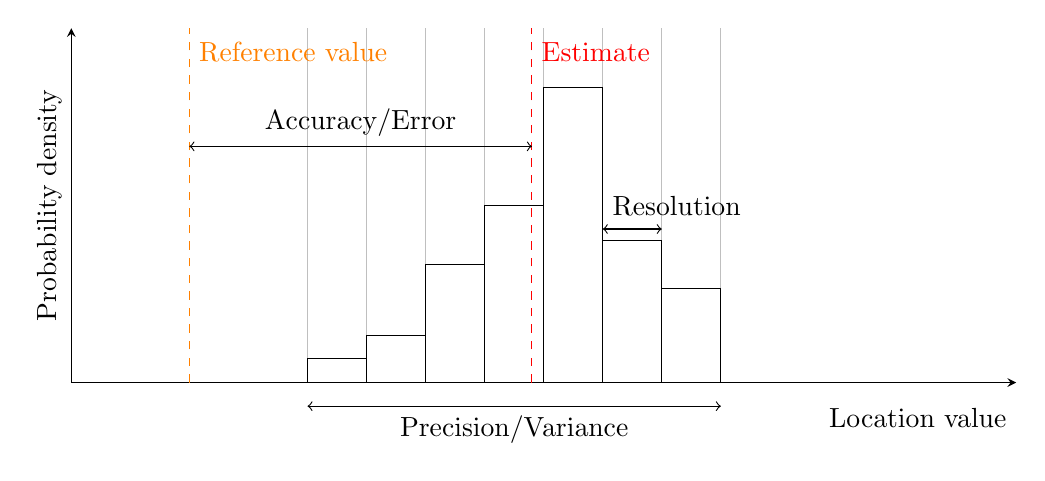
\begin{tikzpicture}

\begin{axis}[
x=1.5cm,
y=1.5cm,
axis y line=left,
axis x line=bottom,
xmax=8,xmin=0,
ymin=0,ymax=3,
xlabel=Location value,
x label style={at={(axis description cs:1,-0.1)},anchor=east},
ylabel=Probability density,
xmajorticks=false,
ymajorticks=false,
width=15cm,
anchor=center,
ybar interval=1,
clip=false
]

\addplot+ [black, fill=white] coordinates {(2,0.2) (2.5,0.4) (3,1) (3.5,1.5) (4,2.5) (4.5,1.2) (5,0.8) (5.5,0.3)};

\draw [dashed, orange] (1,0) -- (1,3);
\node at (1,2.8) [anchor=west, orange] {Reference value};
\draw [dashed, red] (3.9,0) -- (3.9,3);
\node at (3.9,2.8) [anchor=west, red] {Estimate};
\draw [<->, black] (1,2) -- (3.9,2);
\node at (2.45, 2.2) [] {Accuracy/Error};
\draw [<->, black] (4.5, 1.3) -- (5, 1.3);
\node at (4.5, 1.5) [anchor=west] {Resolution};
\draw [<->, black] (2, -0.2) -- (5.5, -0.2);
\node at (3.75, -0.4) [] {Precision/Variance};


\end{axis}
\end{tikzpicture}
\captionof{figure}{Location Terms}
\end{center}